\setlength{\parskip}{\baselineskip}
\section{Architecture Design}

\begin{frame}
	\huge Architecture Design
\end{frame}

\begin{frame}{The platform}
	\begin{itemize}
		\item Targeted for FPGAs
		\item Flexible \& Versatile $\rightarrow$ easy transfer
		\item Scalable $\rightarrow$ multi-FPGA platforms
		\item Expandable $\rightarrow$ Easy adding of new layer types \& accelerators
		\item Capable of running various CNN models
		\item Easy experimentation \& development
		\item Minor to no code changes
	\end{itemize}
\end{frame}

\begin{frame}{Platform Block Diagram}
	\centering
	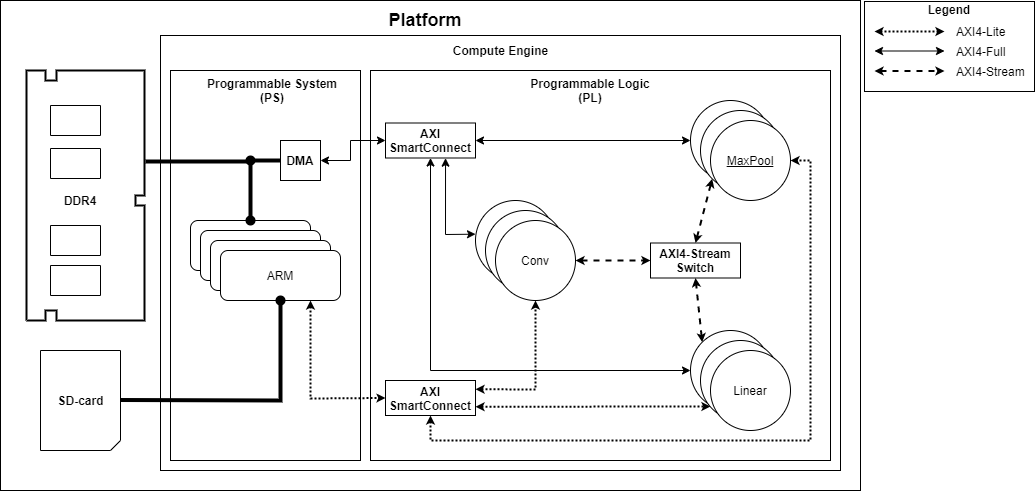
\includegraphics[width=0.9\textwidth]{../Images/Platform/platform-legend-right.png}\\
\end{frame}

\begin{frame}{Platform: Non-Volatile Memory}
	\begin{itemize}
		\item Storage Medium
		\item Network model configurations
		\item Weights \& Biases
		\item Class labels
		\item Input data, e.g. Images
		\item SD card - M.2 SSD (QFDB)
		\item External storage devices via Ethernet \& JTAG
	\end{itemize}
\end{frame}

\begin{frame}{Platform: Volatile Memory}
	\begin{itemize}
		\item Main system memory: DDR
		\item DDR loaded using PS part
		\item No global BRAM module
		\item Accelerators: BRAM caches
		\item Accelerators responsible to load their BRAM \& locate data on DDR
		\item BRAM caches are private to their accelerator
	\end{itemize}
\end{frame}

\begin{frame}{Platform: Compute Engine}
	\begin{itemize}
		\item Both PS \& PL part utilized
		\item Bulk of computation on PL part through hardware accelerators
		\item Sophisticated work on PS part $\rightarrow$ Initialization, Data loading, Input data preprocessing, accelerator configuration \& scheduling
		\item Network layers both software \& hardware
		\item Convolution, Max-Pooling \& Fully-Connected accelerators
		\item Accelerator driver only knows how to configure it
		\item Driver is reusable
	\end{itemize}
\end{frame}

\begin{frame}{Platform: I/O}
	\begin{itemize}
		\item Memory-Mapped I/O (MMIO)
		\item Streaming (AXI4-stream)
		\item BRAM MMIO - Not used
	\end{itemize}
	\centering
	\begin{table}[H]
		\centering
		\begin{tabular}{lll}
			\toprule
			\textbf{Port bit-width} & \textbf{MMIO avg. cycles} & \textbf{Streaming avg. cycles} \\
			\midrule
			32-bit                  & 62700922                  & 65611580                       \\
			128-bit                 & 15761270                  & 16201797                       \\
			\bottomrule
		\end{tabular}
	\end{table}
	40MB data - 40KB bursts
\end{frame}

\begin{frame}{Platform: Software}
	\begin{itemize}
		\item Accelerator drivers - Abstract form, every accelerator implements same functions
		\item Scheduler
		\item Application Logic
		\item User Interface
	\end{itemize}
\end{frame}

\begin{frame}{Platform: Software Flowchart}
	\centering
	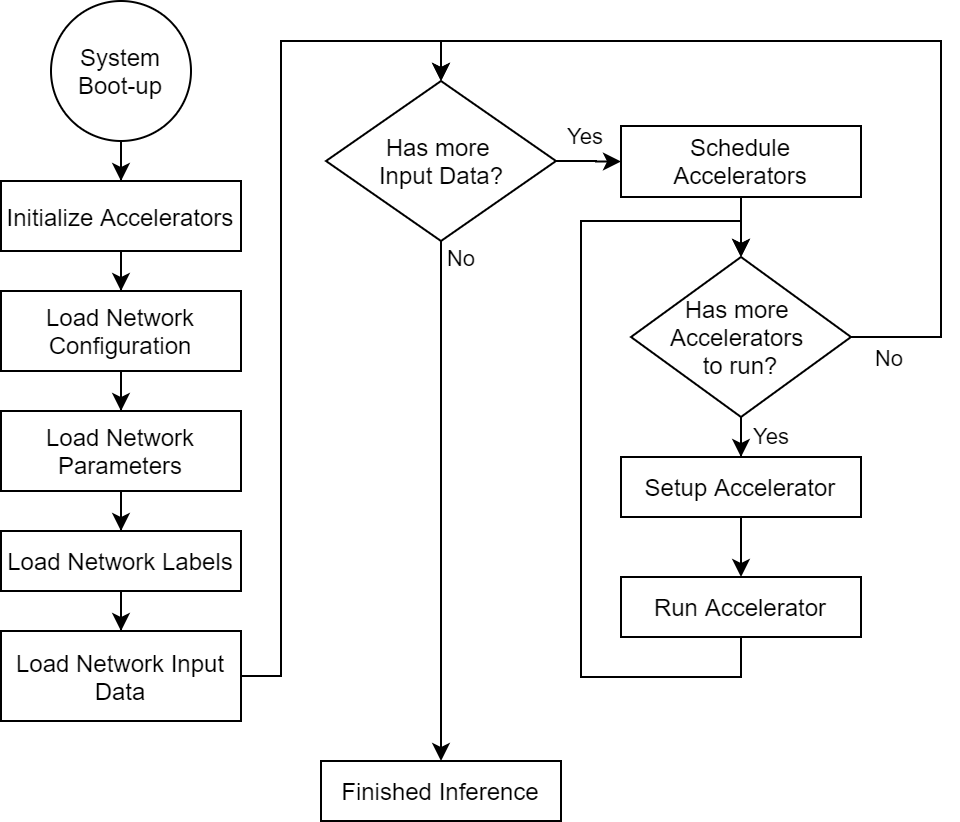
\includegraphics[width=0.5\textwidth]{../Images/Platform/PlatformFlowchart.png}\\
\end{frame}

\begin{frame}{Platform: Serial Scheduler}
	\begin{minipage}{0.6\textwidth}
		\centering
		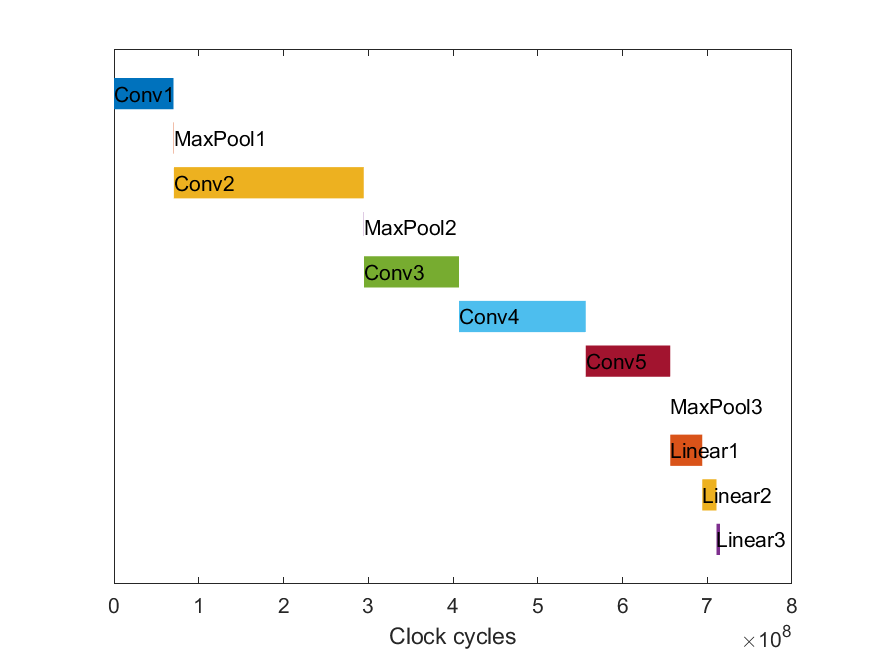
\includegraphics[width=\textwidth]{../Images/Scheduling/Serial.png}\\
	\end{minipage}%
	\begin{minipage}{0.4\textwidth}
		\begin{itemize}
			\item Simple
			\item Best suited for debugging \& validating
			\item About 90\% of total inference time is consumed by convolution layers
			\item Possibility for deadlocks
		\end{itemize}
	\end{minipage}
\end{frame}

\begin{frame}{Platform: Layer Pipelining Scheduler}
	\begin{minipage}{0.6\textwidth}
		\centering
		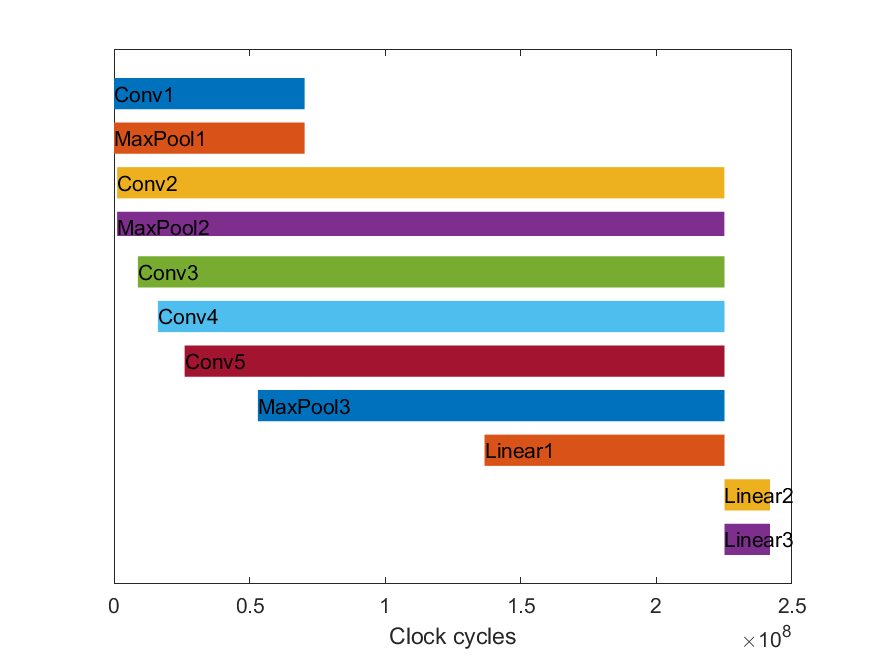
\includegraphics[width=\textwidth]{../Images/Scheduling/Pipelined-1x.png}\\
	\end{minipage}%
	\begin{minipage}{0.4\textwidth}
		\begin{itemize}
			\item A layer gets its input as soon as its previous generates a single output
			\item Accelerator instances needed as many as there are in the model
			\item Almost 3x speedup
			\item Decreases latency \& increases throughput
			\item Accelerators need to support pipelining
			\item Relatively complex
		\end{itemize}
	\end{minipage}
\end{frame}

\begin{frame}{Output Pixel Creation Time}
	\begin{minipage}{0.6\textwidth}
		\centering
		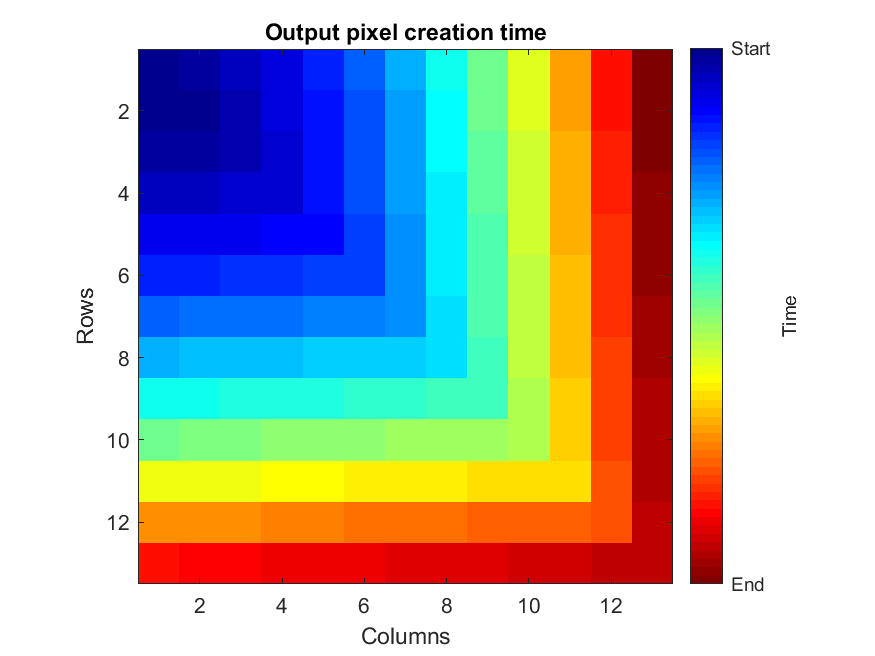
\includegraphics[width=\textwidth]{../Images/Scheduling/Conv5-output-creation-time.png}\\
	\end{minipage}%
	\begin{minipage}{0.4\textwidth}
		\begin{itemize}
			\item Outputs generated in specific order to become useful inputs
			\item Convolution layers use cubes of inputs
			\item Max-Pooling layers use squares of inputs
		\end{itemize}
	\end{minipage}
\end{frame}

\begin{frame}{Pixel Usage Frequency}
	\centering
	\large Larger BRAM caches required\\
	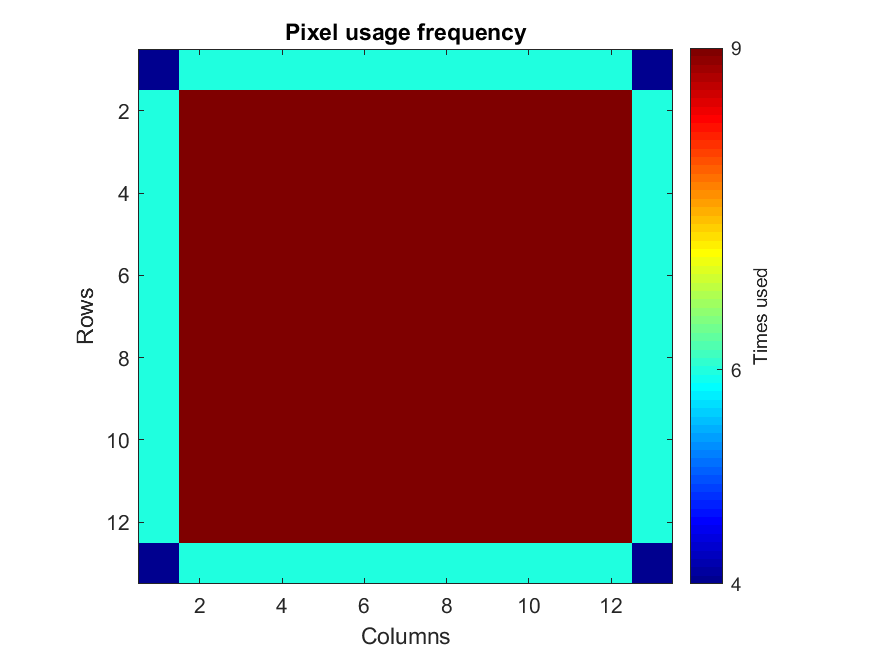
\includegraphics[width=0.45\textwidth]{../Images/Scheduling/Conv5-pixel-frequency.png}
	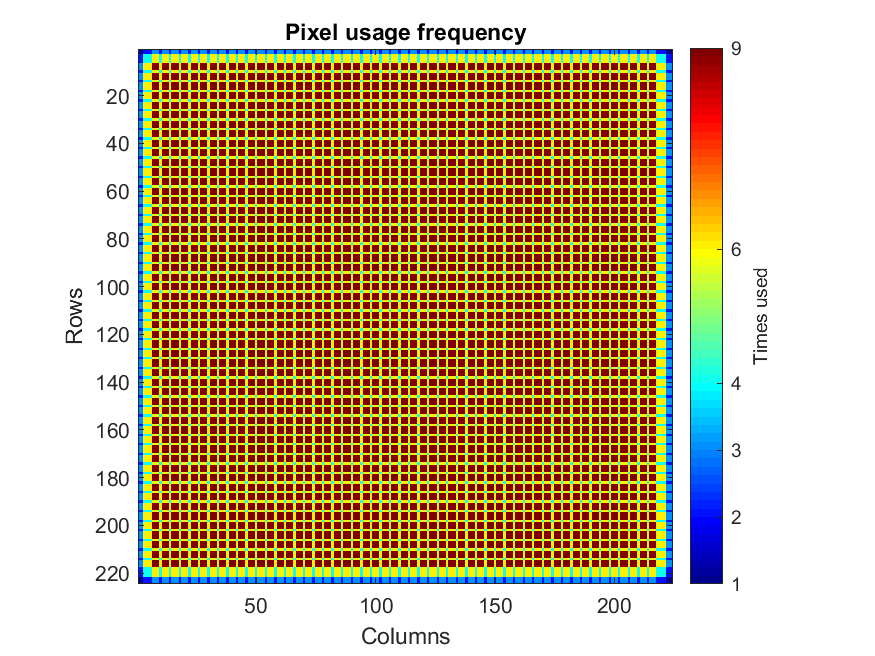
\includegraphics[width=0.45\textwidth]{../Images/Scheduling/Conv1-pixel-frequency.png}\\
\end{frame}

\begin{frame}{Platform: Multi-Inference Scheduler}
	\begin{itemize}
		\item Multiple accelerator instances
		\item Multiple inferences in parallel
		\item Increases batch size \& throughput
		\item Possibility for deadlocks
	\end{itemize}
\end{frame}

\begin{frame}{Platform: Image-Pipelining Scheduler}
	\begin{itemize}
		\item Combination of Layer Pipelining \& Multi-Inference
		\item Every layer handles a different input image
		\item Decreases latency \& increases throughput
		\item Possibility for deadlocks
	\end{itemize}
\end{frame}

\begin{frame}
	\center{\huge{Accelerator Architectures}}
	\begin{itemize}
		\item Two versions: Simple serial \& High performance
		\item Many have been tested
		\item Convolution layer
		\item Max-Pooling layer
		\item Fully-Connected layer
	\end{itemize}
\end{frame}

\begin{frame}{Convolution Accelerator}
	\centering
	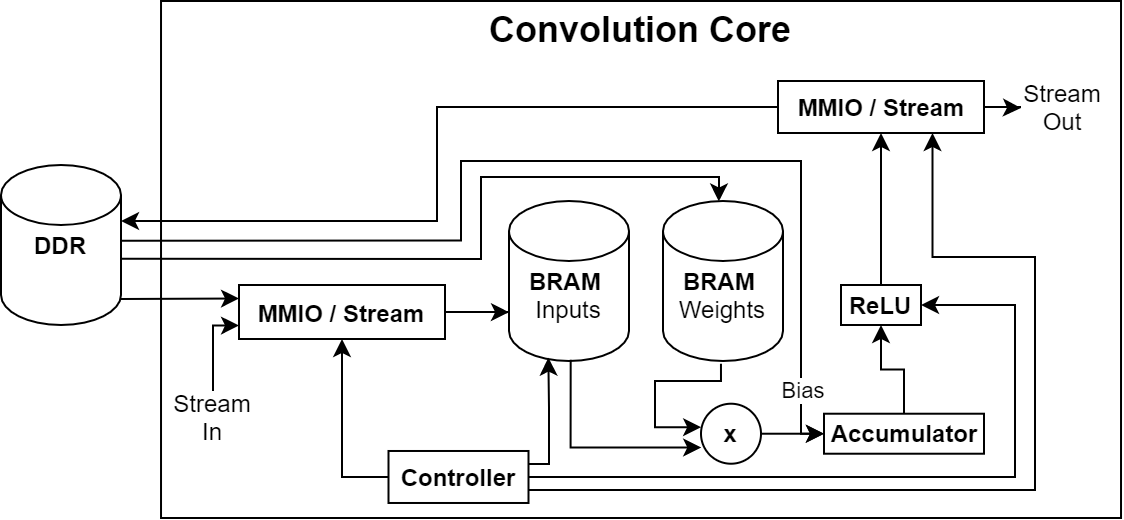
\includegraphics[width=0.7\textwidth]{../Images/Platform/Conv_core_serial.png}\\
\end{frame}

\begin{frame}{Convolution Accelerator}
	\centering
	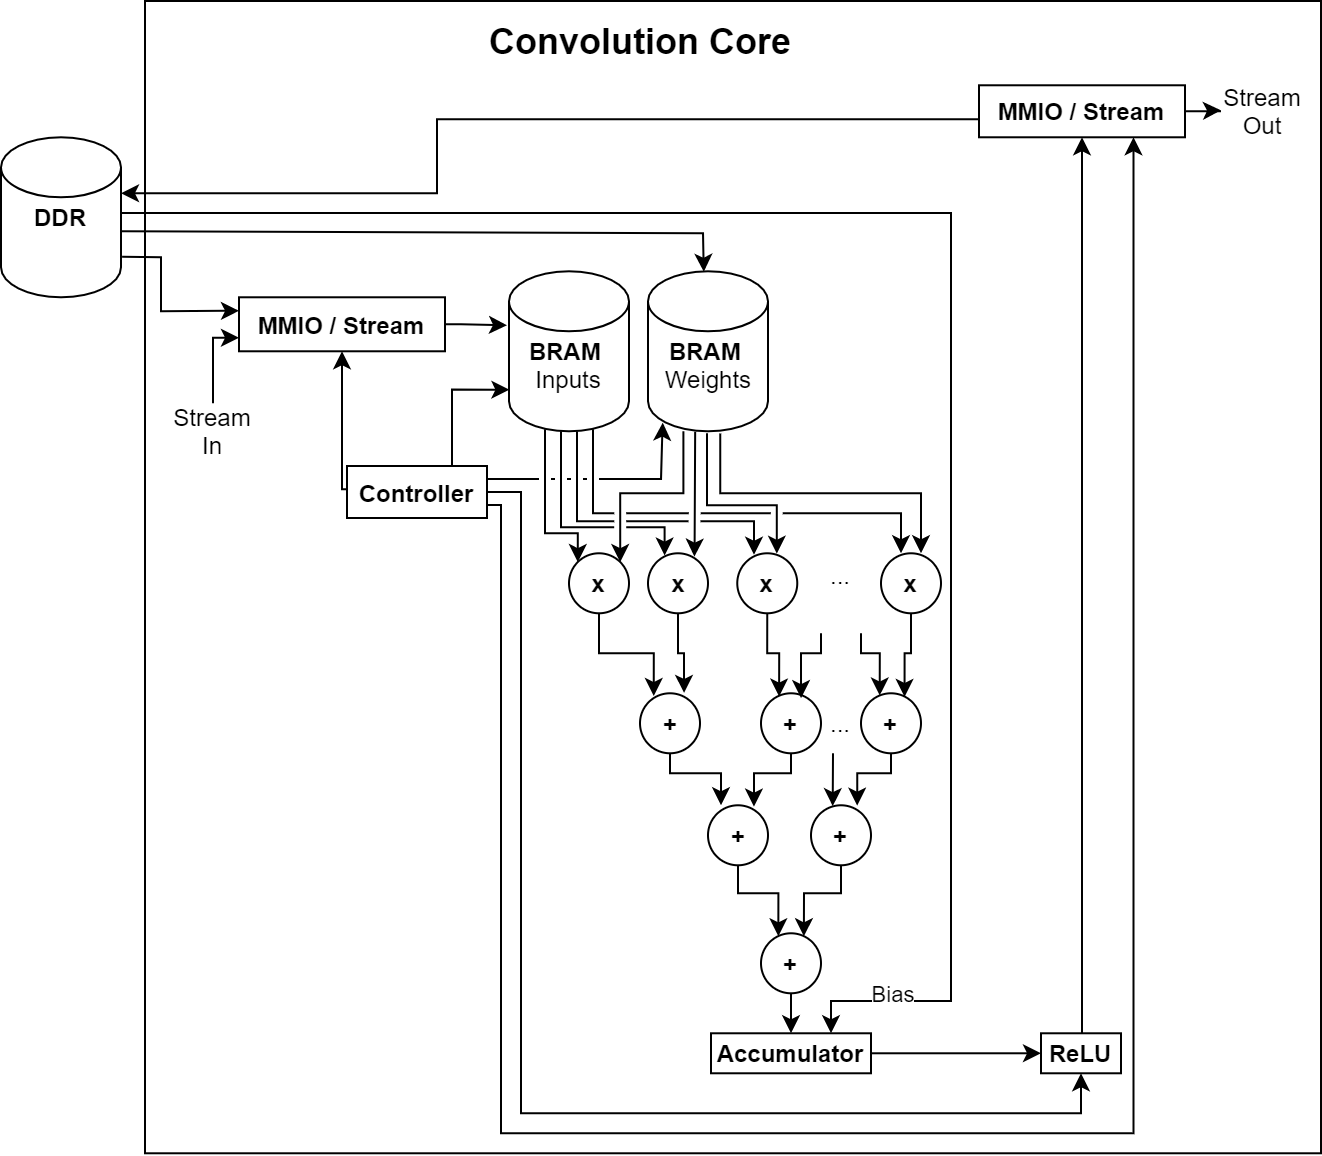
\includegraphics[width=0.5\textwidth]{../Images/Platform/Conv_core_row_parallel.png}\\
\end{frame}

\begin{frame}{ReLU component}
	\centering
	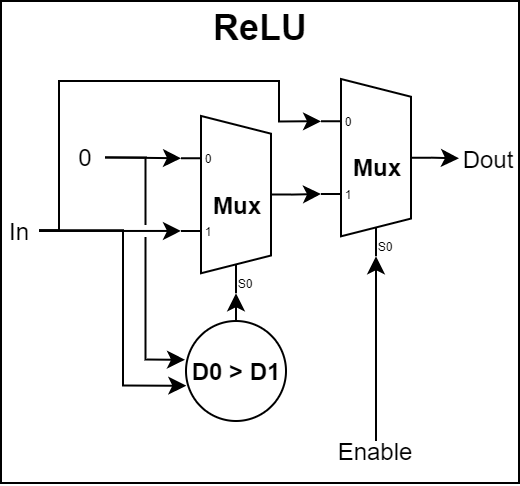
\includegraphics[width=0.4\textwidth]{../Images/Platform/ReLU_component.png}\\
\end{frame}

\begin{frame}{Max-Pooling Accelerator}
	\centering
	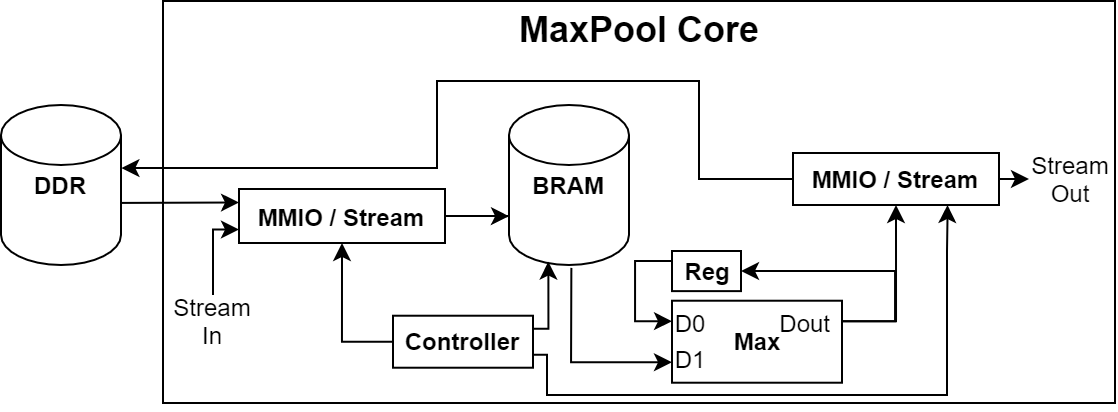
\includegraphics[width=0.9\textwidth]{../Images/Platform/MaxPool_core_serial.png}\\
\end{frame}

\begin{frame}{Max-Pooling Accelerator}
	\centering
	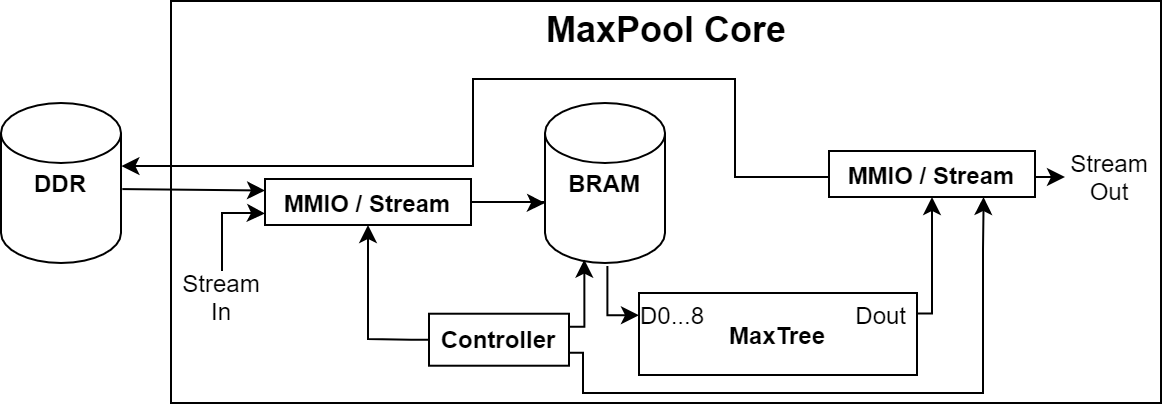
\includegraphics[width=0.9\textwidth]{../Images/Platform/MaxPool_core_kernel_parallel.png}\\
\end{frame}

\begin{frame}{Max \& Max-Tree components}
	\centering
	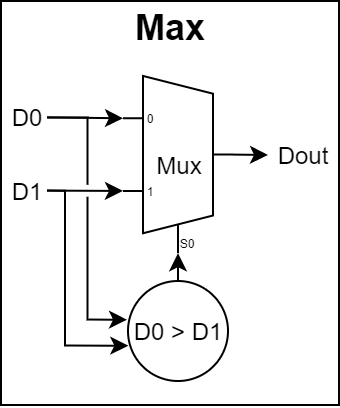
\includegraphics[width=0.2\textwidth]{../Images/Platform/Max_component.png}
	\hspace{0.5cm}
	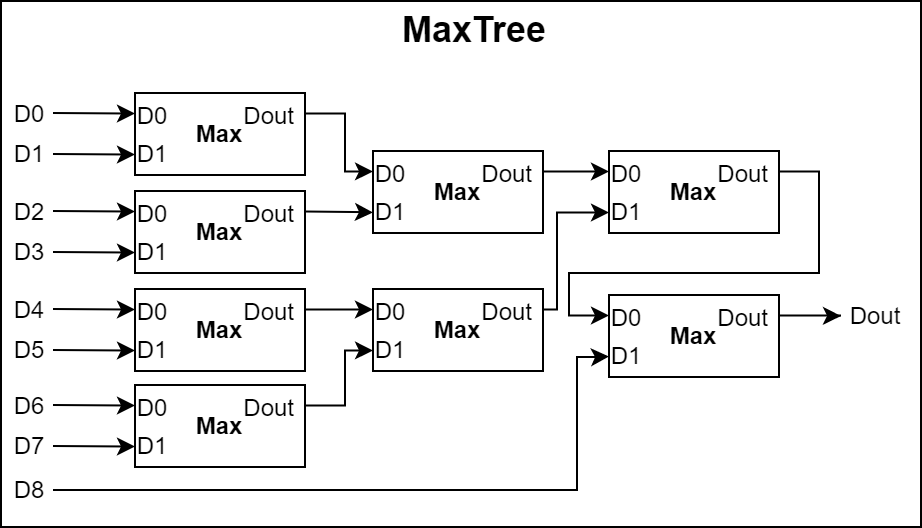
\includegraphics[width=0.7\textwidth]{../Images/Platform/MaxTree_component.png}\\
\end{frame}

\begin{frame}{Fully-Connected Accelerator}
	\centering
	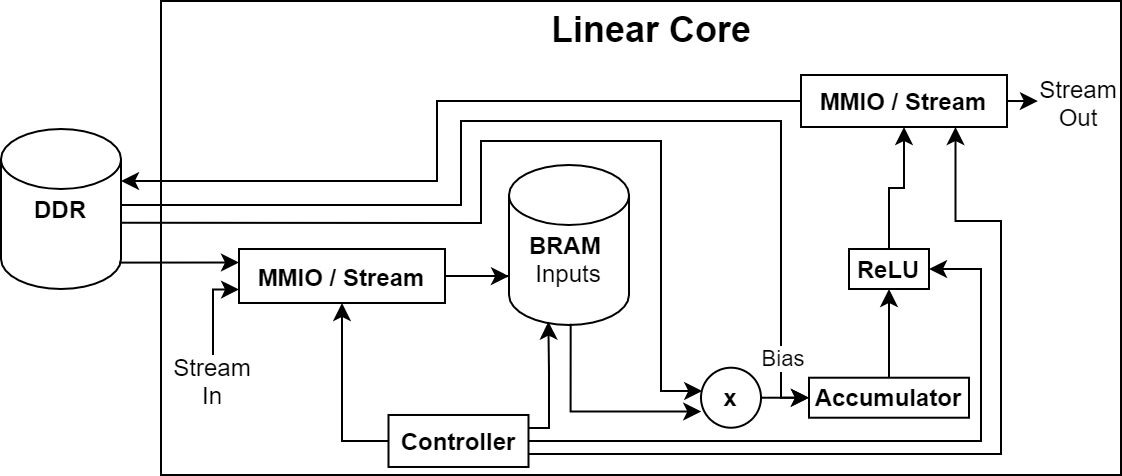
\includegraphics[width=0.9\textwidth]{../Images/Platform/Linear_core_serial.png}\\
\end{frame}

\begin{frame}{Fully-Connected Accelerator}
	\centering
	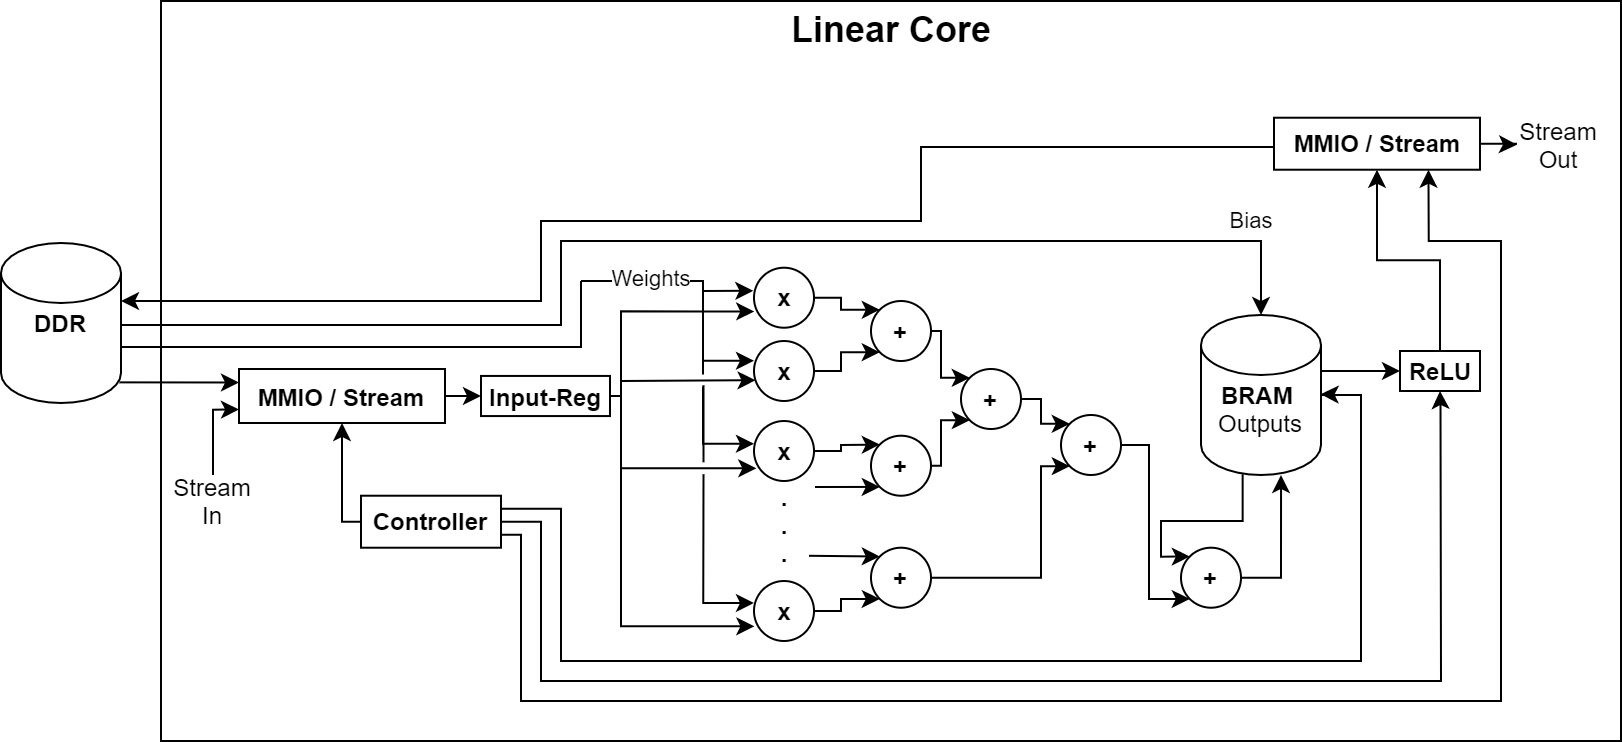
\includegraphics[width=0.9\textwidth]{../Images/Platform/Linear_core_partial_outputs.png}\\
\end{frame}
